\documentclass{beamer}
\usepackage{fprog}

\title{Основни понятия в Haskell}

\date{16 декември 2015 г.}

\begin{document}

\begin{frame}
  \titlepage
\end{frame}

%\includeonlyframes{current}

\section{Въведение в Haskell}

\begin{frame}
  \frametitle{Какво е Haskell?}
  \pause
  \begin{center}
    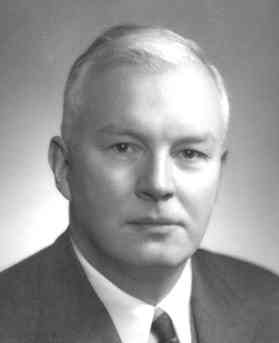
\includegraphics[height=4cm]{images/HaskellBCurry.jpg}\\
    Haskell Brooks Curry\\
    (1900--1982)
  \end{center}
\end{frame}

\begin{frame}[fragile]
  \frametitle{Какво е Haskell?}
  \pause
\begin{verbatim}
fact 0 = 1
fact n = n * fact (n-1)
\end{verbatim}
  \pause
\begin{verbatim}
quickSort []     = []
quickSort (x:xs) = filter (<=x) xs ++ [x] ++ filter (>x) xs
\end{verbatim}
  \pause
\begin{verbatim}
студенти = [("Иван", 40000, 3.5), ("Мария", 60001, 5.5),
            ("Петър", 40002, 5.0), ("Галя", 40003, 4.75)]
избрани = foldr (++) [ ' ':име | (име, фн, оценка) <- оценка,
                                 оценка > 4.5, фн >= 40000 ])
\end{verbatim}
\end{frame}

\begin{frame}
  \frametitle{Какво е Haskell?}
  \pause
  \begin{itemize}
  \item Чист функционален език (без странични ефекти)
  \item Статично типизиран с автоматичен извод на типовете
  \item Използва нестриктно (лениво) оценяване
  \item Стандартизиран (Haskell 2010 Language Report)
  \end{itemize}
\end{frame}

\begin{frame}
  \frametitle{Помощни материали}
  \begin{enumerate}
  \item S. Thompson. Haskell: The Craft of Functional Programming (2nd ed.). Addison-Wesley, 1999.
  \item P. Hudak, Peterson J., Fasel J. A Gentle Introduction to Haskell 98, 1999 (Internet, 2008).
  \item Haskell Wiki: \url{https://wiki.haskell.org/Haskell}
  \item Haskell Platform: \url{https://www.haskell.org/platform/}
  \end{enumerate}
\end{frame}

\section{Дефиниции}

\begin{frame}
  \frametitle{Синтактични елементи}
  \begin{itemize}
  \item Идентификатори: \tt{fact}, \tt{\_myvar}, \tt{студенти}
    \begin{itemize}
    \item имена на обекти, започват с малка буква или \tt\_
    \end{itemize}
  \item Запазени идентификатори: \tt{case}, \tt{if}, \tt{let}, \tt{where}, \ldots
  \item Конструктори: \tt{Integer}, \tt{Maybe}, \tt{Just}, \ldots
    \begin{itemize}
    \item имена на конструкции, започват с главна буква
    \end{itemize}
  \item Числа: \tt{10}, \tt{-5.12}, \tt{3.2e+2}, \tt{1.2E-2}, \tt{0x2f}, \tt{0o35}
  \item Операции: \tt+, \tt*, \tt{\&\%}, \tt{<==>}, \tt{$\spadesuit$}
    \begin{itemize}
    \item поредица от символи (без букви и цифри)
    \item всички операции с изключение на унарния \tt- са инфиксни
    \end{itemize}
  \item Запазени операции: \tt{..} \tt: \tt{::} \tt= \tt\textbackslash \tt| \tt{<-} \tt{->} \tt@ \tt\~ \tt{=>}
  \item Специални символи: \tt( \tt) \tt, \tt; \tt[ \tt] \tt` \tt\{ \tt\}
  \item Знаци: \tt{'a'}, \tt{'\textbackslash n'}, \tt{'+'}
  \item Низове: \tt{"Hello, world!"}, \tt{"произволен низ"}
  \end{itemize}
\end{frame}

\begin{frame}
  \frametitle{Декларации и дефиниции}
  \begin{itemize}[<+->]
  \item {}<име> \tta{::} <тип> (типова декларация)
  \item декларира се, че <име> ще се свързва със стойности от <тип>
  \item \alert{типовите декларации са незадължителни: в повечето случаи Haskell може сам да се ориентира за правилния тип}
    \begin{itemize}[<.->]
    \item \tt{x :: Int}
    \item \tt{y :: Double}
    \item \tt{z :: String}
    \end{itemize}
  \item {}<име> \tta= <израз> (дефиниция)
  \item {}<име> се свърза с <израз>
    \begin{itemize}[<.->]
    \item \tt{x = 2}
    \item \tt{y = x\^{}2 + 7.5}
    \item \tta{z = x + y}
    \item \tt{z = "Hello"}
    \end{itemize}
  \end{itemize}
\end{frame}

\begin{frame}
  \frametitle{Типове}
  Типовете в Haskell обикновено се задават с конструктори. \pause
  \begin{itemize}[<+->]
  \item \tt{Bool} --- булев тип с константи \tt{True} и \tt{False}
  \item \tt{Char} --- Unicode знаци
  \item Целочислени
    \begin{itemize}
    \item \tt{Int} --- цели числа с фиксирана големина $[-2^{63}; 2^{63}-1]$
    \item \tt{Integer} --- цели числа с произволна големина
    \end{itemize}
  \item С плаваща запетая
    \begin{itemize}
    \item \tt{Float} --- дробни числа с единична точност
    \item \tt{Double} --- дробни числа с двойна точност
    \end{itemize}
  \item Съставни
    \begin{itemize}
    \item \tt{[a]} --- тип списък с \textbf{произволна} дължина и
      елементи от \textbf{фиксиран} тип \tt a
    \item \tt{String = [Char]} --- низ (списък от знаци)
    \item \tt{(a,b,c)} --- тип кортеж (наредена $n$-торка) с
      \textbf{фиксирана} дължина и \textbf{произволни} типове на
      компонентите
    \end{itemize}
  \end{itemize}
\end{frame}

\section{Вградени функции и операции}

\begin{frame}
  \frametitle{Стандартен модул \tt{Prelude}}
  \begin{itemize}[<+->]
  \item програмите в Haskell се разделят на модули
  \item \tta{module} <име> \tta{where}
  \item дефинира модул с <име>
  \item \tta{import} <модул>[\tta.<име>]
  \item внася дефиницията <име> от <модул>
  \item ако <име> не е указана, внася всички дефиниции
  \item стандартната библиотека в Haskell се съдържа в модула \tt{Prelude}
  \item всички дефиниции от \tt{Prelude} се внасят автоматично във всяко програма
  \end{itemize}
\end{frame}

\begin{frame}
  \frametitle{Стандартни числови функции}

  Аритметични операци

  \tt{+}, \tt{-}, \tt{*}, \tt{/}, \tt{\^{}}, \tt{\^{}\^{}}

  \vspace{1em}
  Други числови функции

  \tt{div}, \tt{mod}, \tt{max}, \tt{min}, \tt{gcd}, \tt{lcm}

  \vspace{1em}
  Функции за преобразуване

  \tt{fromInteger}, \tt{fromRational}, \tt{round}, \tt{ceiling}, \tt{floor}

  \vspace{1em}
  Функции над дробни числа

  \tt{exp}, \tt{log}, \tt{sin}, \tt{cos}, \tt{tan}, \tt{asin}, \tt{acos}, \tt{atan}, \tt{sqrt}, \tt{**}
\end{frame}

\begin{frame}
  \frametitle{Стандартни предикати}

  Числови предикати

  \tt{<}, \tt{>}, \tt{=}, \tt{/=}, \tt{<=}, \tt{>=}, \tt{odd}, \tt{even}

  \vspace{1em}
  Булеви операции

  \tt{\&\&}, \tt{||}, \tt{not}
\end{frame}

\section{Функции}

\begin{frame}
  \frametitle{Функции в Haskell}
  \begin{itemize}[<+->]
  \item \tt{t1 -> t2} --- тип на функция, която получава параметър от тип \tt{t1} и връща резултат от тип \tt{t2}
  \item {}<име> <параметър> \tta= <тяло>
  \item дефиниция на функция с <име>, един <параметър> и <тяло>
  \item {}<функция> <израз>
  \item прилагане на <функция> над <израз>
    \begin{itemize}[<.->]
    \item \tt{square :: Int -> Int}
    \item \tt{square x = x * x}
    \item \evalsto{square x}4
    \item \evalstoerr{square 2.7}
    \end{itemize}
  \item \alert{Прилагането е с по-висок приоритет от другите операции!}
  \item \evalsto{square 2 + 3}7
  \item \evalsto{square (2 + 3)}{25}
  \end{itemize}
\end{frame}

\begin{frame}
  \frametitle{Функции на повече параметри}
  \begin{itemize}[<+->]
  \item Как можем да изразим функция $f(x,y)$ на два параметъра чрез функции с един параметър?
  \item Разглеждаме функция $F$ на един параметър $x$,...
  \item ...която връща като резултат функцията на един параметър $f_x$,...
  \item ...така че $f_x(y) = f(x,y)$.
  \item Така имаме $f(x,y) = F(x)(y)$.
  \end{itemize}
  \pause
  \begin{block}{Основна идея}
    Можем да разглеждаме функции с $n$ параметъра, като функции с един параметър, които връщат функции с $n-1$ параметъра.
  \end{block}
  \pause
  \alert{Това преобразува над функциите с повече параметри се нарича ``къринг'' (``currying'').}
\end{frame}

\begin{frame}
  \frametitle{Currying в Haskell}
  \begin{itemize}[<+->]
  \item \tt{t1 \alert{->} (t2 \alert{->} t3)}
    \begin{itemize}
    \item функция с параметър от тип \tt{t1}, която връща функция, която приема параметър от тип \tt{t2} и връща резултат от тип \tt{t3}; или
    \item функция на два параметъра от типове \tt{t1} и \tt{t2}, която връща резултат от тип \tt{t3}
    \end{itemize}
  \item В общия случай: <функция> \tt{\alert{::} t1 \alert{->} (t2 \alert{->}} \ldots \tt{(tn \alert{->} t)}\ldots\tt)
  \item{} <функция> ще очаква $n$ параметъра от типове \tt{t1}, \tt{t2}, \ldots, \tt{tn} и ще връща резултат от тип \tt{t}
  \item{} <функция> <параметър$_1$> \ldots <параметър$_n$> \tt= <тяло>
  \item дефинира <функция> с $n$ параметъра и <тяло>
    \begin{itemize}
    \item \tt{hypothenuse :: Double -> Double -> Double}
    \item \tt{hypothenuse a b = sqrt (square a + square b)}
    \item \evalsto{\alt<+->{hypothenuse 3 4}{(hypothenuse 3) 4}}5
    \end{itemize}
  \end{itemize}
\end{frame}

\begin{frame}<1-6>
  \frametitle{Частично прилагане на функции}
  Кърингът позволява удобно прилагане на функция към само част от параметрите.
  \begin{itemize}[<+->]
  \item \tt{div50 :: Int -> Int}
  \item \tt{div50\temporal<4>{ x}{ $\not{\tt x}$}{} = div 50\temporal<4>{ x}{ $\not{\tt x}$}{}}
  \item \evalsto{div50 4}{12}
  \end{itemize}
\end{frame}

\begin{frame}
  \frametitle{Функции от по-висок ред}
  \alert{Внимание:} \tt{t1 -> (t2 -> t3)} $\neq$ \tt{(t1 -> t2) -> t3}!\pause
  \begin{itemize}[<+->]
  \item операцията \tt{->} е \textbf{дясноасоциативна}
  \item \tt{t1 -> (t2 -> t3)} $\equiv$ \tt{t1 -> t2 -> t3}
  \item \tt{(t1 -> t2) -> t3} --- функция, която връща резултат от тип \tt{t3}, а приема като единствен параметър функция, която приема един параметър от тип \tt{t1} и връща резултат от тип \tt{t2}
  \item \alert{функция от втори ред}
    \begin{itemize}
    \item \tt{twice :: (Int -> Int) -> Int -> Int}
    \item \tt{twice f x = f (f x)}
    \item \evalstop{twice square 3}{81}
    \item \evalstop{twice (mod 13) 5}1
    \item \tt{diag f x = f x x}
    \item \tt{diag :: (Int -> Int -> Int) -> Int -> Int}
    \item \evalstop{diag div 5}1
    \item \evalstop{diag hypothenuse 1}{1.4142135623730951}
    \item \tt{diag :: (t1 -> t1 -> t) -> t1 -> t}
    \end{itemize}
  \end{itemize}
\end{frame}

\begin{frame}
  \frametitle{Функции и операции}
  \begin{itemize}[<+->]
  \item Функциите в Haskell са винаги с \textbf{префиксен} запис
  \item Операциите в Haskell са винаги \textbf{бинарни с инфиксен}
    запис.
    \begin{itemize}
    \item \alert{Изключение:} унарен минус: \tt{-a}
    \item \evalstoerr{square -x}
    \item \evalsto{square (-x)}4
    \end{itemize}
  \item Преобразуване на бинарни функции към операции: \tta`<функция>\tta`
    \begin{itemize}
    \item \evalsto{13 `div` 5}3
    \item \evalstoerr{2 `square`}
    \end{itemize}
  \end{itemize}
\end{frame}

\begin{frame}
  \frametitle{Операции и функции}
  \begin{itemize}[<+->]
  \item Преобразуване на операции към бинарни функции: \tta(<операция>\tta)
    \begin{itemize}
    \item \evalsto{(+) 2 3}5
    \item \tt{plus1 = (+) 1}
    \item \tt{square = diag (*)}
    \end{itemize}
  \item Преобразуване на операции към унарни функции (секция на операции)
    \begin{itemize}
    \item \tta(<израз> <операция>\tta) --- лява секция
    \item \tta(<операция> <израз>\tta) --- дясна секция
    \item \evalstop{(2\^{}) 3}8
    \item \evalstop{(\^{}2) 3}9
    \item \tt{square = (\^{}2)}
    \item \evalstoerrp{(-5) 8}
    \item \evalstop{twice (*2) 5}{20}
    \item \tt{positive = (>0)}
    \item \tt{lastDigit = (`mod` 10)}
    \end{itemize}
  \end{itemize}
\end{frame}

\section{Условни операции}

\begin{frame}
  \frametitle{\tt{if} \ldots \tt{then} \ldots \tt{else}}
  \begin{itemize}[<+->]
  \item \tta{if} <условие> \tta{then} <израз$_1$> \tta{else} <израз$_2$>
    \begin{itemize}[<.->]
    \item Ако <условие> е \tt{True}, връща <израз$_1$>
    \item Ако <условие> е \tt{False}, връща <израз$_2$>
    \end{itemize}
  \item \tt{abs x = if x < 0 then -x else x}
  \item \tt{fact n = if n == 0 then 1 else n * fact (n - 1)}
  \item \evalstoerr{if x > 5 then x + 2 else "Error"}
  \item \alert{<израз$_1$> и <израз$_2$> трябва да са от един и същи тип!}
  \item \alert{<условие> трябва да е от тип \tt{Bool}!}
  \end{itemize}
\end{frame}

\begin{frame}[fragile]
  \frametitle{Разглеждане на случаи}
  Дефинниране на функции с разглеждане на случаи.
  \begin{itemize}
    \item{} <име> \{<параметър>\}\\
      \hspace{3ex} \{ \tta| <пазач> \tta= <израз> \}
    \item{} <име> <параметър$_1$> <параметър$_2$> ... <параметър$_k$>\\
      \hspace{3ex} \tta| <пазач$_1$> \tta= <израз$_1$>\\
      \ldots\\
      \hspace{3ex} \tta| <пазач$_n$> \tta= <израз$_n$>\\
  \item ако <пазач$_1$> е \tt{True} връща <израз$_1$>, а ако е \tt{False}:
  \item \ldots
  \item ако <пазач$_n$> е \tt{True} връща <израз$_n$>, а ако е \tt{False}:
  \item \alert{грешка!}
  \item За удобство \tt{Prelude} дефинира \tt{otherwise = True}
  \end{itemize}
\end{frame}

\begin{frame}[fragile]
  \frametitle{Разглеждане на случаи --- примери}
\begin{verbatim}
fact n
  | n == 0    = 1
  | n > 0     = n * fact (n - 1)
  | n < 0     = 0
\end{verbatim}
\pause\vspace{1em}
\begin{verbatim}
grade x
  | x >= 5.5    = "Отличен"
  | x >= 4.5    = "Много добър"
  | x >= 3.5    = "Добър"
  | x >= 3      = "Среден"
  | otherwise   = "Слаб"
\end{verbatim}
\end{frame}

\section{Вложени дефиниции}

\begin{frame}
  \frametitle{Локални дефиниции с \tt{let}}
  \begin{itemize}
  \item \tta{let} \{ <име> \tta= <израз> \}\\
    \tta{in} <тяло>
  \item \tta{let} <име$_1$> \tta= <израз$_1$>\\
    \hspace{5ex}<име$_2$> \tta= <израз$_2$>\\
    \hspace{5ex}\ldots\\
    \hspace{5ex}<име$_n$> \tta= <израз$_n$>\\
    \tta{in} <тяло>
  \item дефинициите <име$_i$> = <израз$_i$> се въвеждат едновременно само за оценката на <тяло>
  \item дефинициите може да са взаимно рекурсивни
  \item редът на дефинициите е без значение
  \end{itemize}
\end{frame}

\begin{frame}
  \frametitle{Локални дефиниции с \tt{where}}
  \begin{itemize}
  \item{} <функция> \{ <параметри> \} = <тяло>\\
        \hspace{5ex} \tta{where} \{ <име> \tta= <израз> \}
  \item{} <функция> <параметър$_1$> \ldots <параметър$_k$> = <тяло>\\
        \hspace{5ex} \tta{where} <име$_1$> \tta= <израз$_1$>\\
        \hspace{11ex} <име$_2$> \tta= <израз$_2$>\\
        \hspace{11ex}\ldots\\
        \hspace{11ex} <име$_n$> \tta= <израз$_n$>\\
  \item дефинициите <име$_i$> = <израз$_i$> се въвеждат едновременно само за оценката на <тяло>
  \item дефинициите може да са взаимно рекурсивни, редът е без значение
  \end{itemize}
\end{frame}

\begin{frame}[fragile]
  \frametitle{Локални дефиниции --- пример}
\begin{verbatim}
area x1 y1 x2 y2 x3 y3 =
   let a = dist x1 y1 x2 y2
       b = dist x2 y2 x3 y3
       c = dist x3 y3 x1 y1
       p = (a + b + c) / 2
   in sqrt (p * (p - a) * (p - b) * (p - c))
   where dist u1 v1 u2 v2 = sqrt (du^2 + dv^2)
          where du = u2 - u1
                dv = v2 - v1
\end{verbatim}
\end{frame}

\end{document}
